\section{User Manual}
When launching Minion Map, you will be greeted by a welcome-screen where the following launch options are provided. Launching Copenhagen, Bornholm or selecting your own file to display in the program by dragging and dropping the file into the program. Alternatively, you can manually navigate to a file in File Explorer by pressing Open Filefinder, choosing the file and confirming your choice by pressing “Launch Map”.
\begin{figure}[ht]%
  \centering
  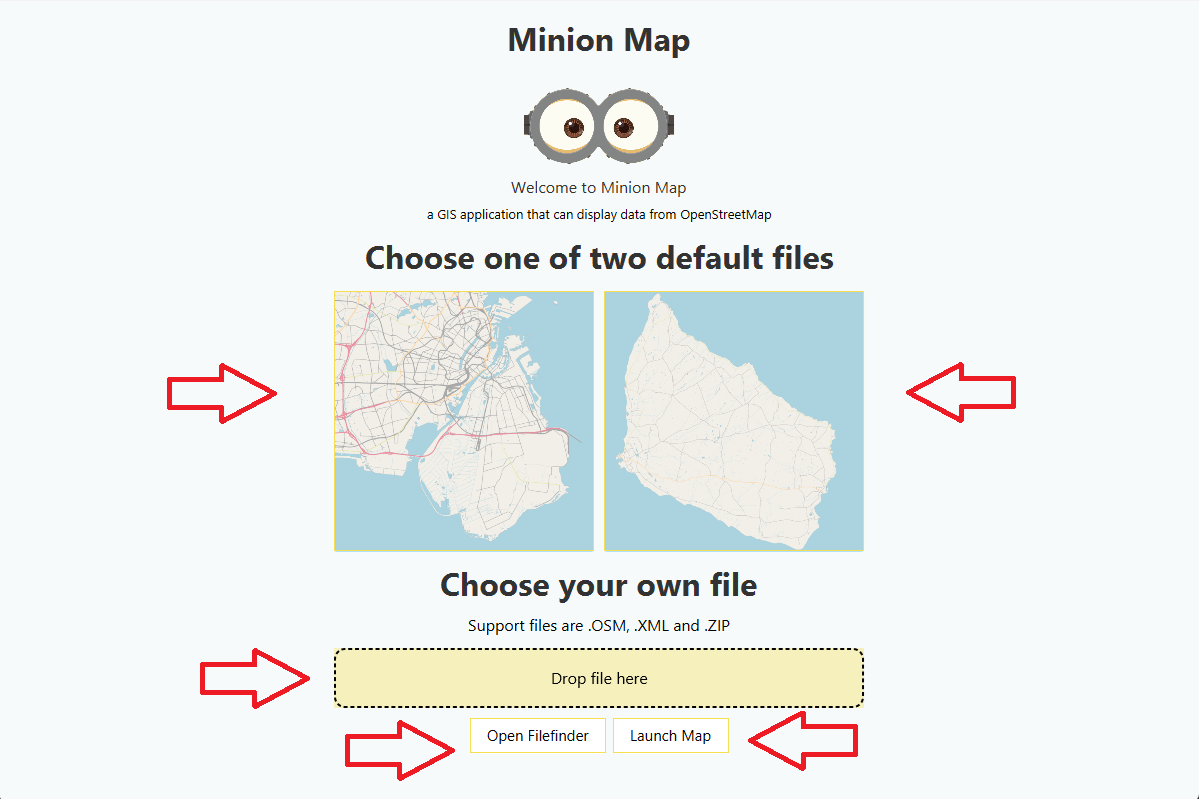
\includegraphics[width=14.5cm]{docs/material/UserManual_Start.png}%
\end{figure}\\
This will take you to the loaded map of your choice, providing you with options such as address finder, pathfinding, point of interest marking and theme chooser. 
Finding an address is done by selecting and typing in the textfield found at the top of the screen.
\begin{figure}[ht]%
  \centering
  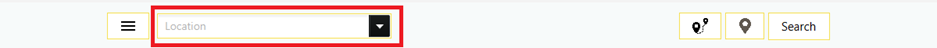
\includegraphics[width=14.5cm]{docs/material/UserManual_AddressSearch.png}%
\end{figure}
\newpage
As you type in your address, you will dynamically give suggestions, saving you from typing the rest of the address. When the correct address is selected, the map will pan to your requested destination. 
\begin{figure}[ht]%
  \centering
  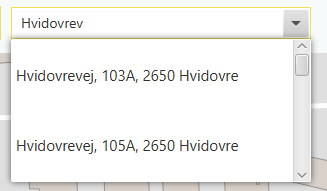
\includegraphics[width=5.5cm]{docs/material/AddressSearchDropdown1.png}%
\end{figure}\\
Pathfinding between to addresses can be done by pressing the “Route" button found at the leftmost location of the three buttons in the upper right corner. 
\begin{figure}[ht]%
  \centering
  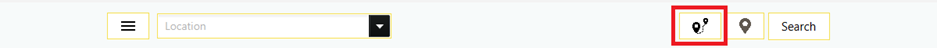
\includegraphics[width=14.5cm]{docs/material/UserManual_RouteButton.png}%
\end{figure}\\
From here on you type in your two addresses that you wish to find a path between and press "Enter" or the "Find Route" button.
\begin{figure}[ht]%
  \centering
  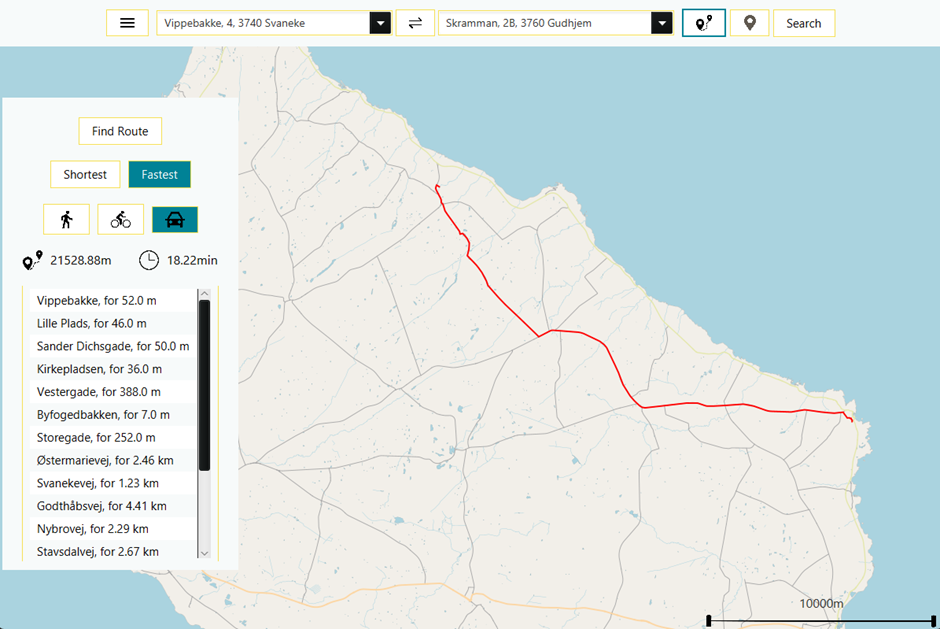
\includegraphics[width=13.5cm]{docs/material/UserManual_Pathfinding.png}%
\end{figure}\\
Also provided is the Transportation menu, giving you options such as quickest or shortest path and choice of transportation. You will also be provided with a route guide, distance of the route and minutes of travel.

The feature for changing the color theme is found in the "Hamburger" menu in the upper left corner of the screen. Press that and you will find a dropdown menu displaying your options. 
